
%%%%%%%%%%%%%%%%%%%%%%% file typeinst.tex %%%%%%%%%%%%%%%%%%%%%%%%%
%
% This is the LaTeX source for the instructions to authors using
% the LaTeX document class 'llncs.cls' for contributions to
% the Lecture Notes in Computer Sciences series.
% http://www.springer.com/lncs       Springer Heidelberg 2006/05/04
%
% It may be used as a template for your own input - copy it
% to a new file with a new name and use it as the basis
% for your article.
%
% NB: the document class 'llncs' has its own and detailed documentation, see
% ftp://ftp.springer.de/data/pubftp/pub/tex/latex/llncs/latex2e/llncsdoc.pdf
%
%%%%%%%%%%%%%%%%%%%%%%%%%%%%%%%%%%%%%%%%%%%%%%%%%%%%%%%%%%%%%%%%%%%


\documentclass[runningheads,a4paper]{llncs}

\usepackage{amssymb}
\setcounter{tocdepth}{3}
\usepackage{graphicx}
\usepackage{lipsum}

\usepackage{url}
\urldef{\mailsa}\path|{alfred.hofmann, ursula.barth, ingrid.haas, frank.holzwarth,|
\urldef{\mailsb}\path|anna.kramer, leonie.kunz, christine.reiss, nicole.sator,|
\urldef{\mailsc}\path|erika.siebert-cole, peter.strasser, lncs}@springer.com|    
\newcommand{\keywords}[1]{\par\addvspace\baselineskip
\noindent\keywordname\enspace\ignorespaces#1}

\begin{document}

\mainmatter  % start of an individual contribution

% first the title is needed
\title{Babbage, Ada y la Máquina Analítica}

% a short form should be given in case it is too long for the running head
\titlerunning{Babbage, Ada y la Máquina Analítica}

% the name(s) of the author(s) follow(s) next
%
% NB: Chinese authors should write their first names(s) in front of
% their surnames. This ensures that the names appear correctly in
% the running heads and the author index.
%
\author{Carlos Rafael Ortega Lezcano \and Eric Martín García}
%
\authorrunning{Babbage, Ada y la Máquina Analítica}
% (feature abused for this document to repeat the title also on left hand pages)

% the affiliations are given next; don't give your e-mail address
% unless you accept that it will be published
\institute{Universidad de la Habana}

%
% NB: a more complex sample for affiliations and the mapping to the
% corresponding authors can be found in the file "llncs.dem"
% (search for the string "\mainmatter" where a contribution starts).
% "llncs.dem" accompanies the document class "llncs.cls".
%

\toctitle{Babbage, Ada y la Máquina Analítica}
\tocauthor{Authors' Instructions}
\maketitle


\begin{abstract}
Ada Lovelace trabajó junto a Charles Babbage para crear una descripción de la máquina analítica creada por Babbage 
usando como inspiración la fallida máquina de diferencias. Era una calculadora automatizada la cual podía realizar
operaciones aritmética cuya característica más relevante era el hecho de ser programable, convirtiendo a sus creadores
en pioneros del desarrollo de la computación que se daría con posterioridad en el siglo XX. Este trabajo recopila aspectos bibliográficos de la vida de ambos además que explica la composición y funcionamiento de la máquina y como era posible programarla siguiendo lo expuesto por Ada Lovelace en 1843.
\end{abstract}


\section{Introducción}

La máquina analítica de Charles Babbage es un extraordinario avance conceptual y mecánico ocurrido
entre los años 1834 y 1847, este diseñó los planos y mecanismos de una máquina calculadora programable, 
que era un extraordinario avance conceptual y mecánico para su época el cual queda desaprovechado
por la cultura circundante durante unos cien años. No sería hasta la 2da Guerra Mundial que tendría lugar
un proceso científico y económico mediante un creciente perfeccionamiento tecnológico e industrial, 
que lo colocó en diversos sectores de la sociedad, dando lugar a la sociedad de la información, y al desarrollo de los ordenadores personales.

Babbage investigó múltiples opciones para la máquina analítica y perfeccionó el diseño en varias direcciones
diferentes, por lo tanto, escogeremos una parte del trabajo, en particular, el desarrollado hacia 1838. 
Durante esta etapa media de la evolución de la máquina analítica ya se muestran sus atributos principales 
y definitivos, aunque en una forma que será simplificada durante los años siguientes.

La primera mención de la máquina analítica fue hecha en 1834, en una carta enviada por Babbage al 
duque de Wellington, primer ministro en aquel año. La primera descripción profunda de dicha máquina, 
fue en 1837, a mitad de año, en un manuscrito entregado por Babbage a su amigo H. W. Buxton, quien 
tenía intención de escribir una historia sobre sus máquinas, sin embargo, la mejor descripción contemporánea 
sería la extensa traducción y las notas escritas (bajo la supervisión y consejo de Babbage) por Ada 
Lovelace del artículo de ingeniería descriptiva compuesto en italiano por Luigi Menabrea, con ocasión 
de la estancia de Babbage en Turín, al cual Babbage añadió algunas explicaciones, estas notas confeccionadas 
por Ada Lovelace fueron publicadas en el \emph{Taylor’s Scientific Memoirs} en 1843 bajo el titulo de 
\emph{Notes}, en este año se tenía ya una idea clara y simplificada de la máquina analítica. 
Además de esto, Babbage en 1864 mientras escribía su autobiografía dedicó un capítulo de ésta a la 
máquina analítica.

\section{Sobre los creadores}

La confección de la máquina analítica por Charles Babbage y los escritos sobre la configuración de la misma por Ada Lovelace son parte importante en el desarrollo de la computación, es necesario por tanto conocer el devenir de sus creadores, el contexto en el cual se desarrollaron y el impacto que pudo tener la máquina analítica en el resto de
sus trabajos.

\subsubsection{Augusta Ada Byron King (1815 - 1852):} Ada Byron, nació en Londres el 10 de diciembre de 1815, hija de Annabela Noel-Byron y del famoso poeta Lord Byron. Ada Bayron tuvo una educación privilegiada como pocas mujeres en el siglo XIX, disfrutando desde niña de un alto nivel socioeconómico. Tuvo acceso a tutores privados de la sociedad literaria y científica del Reino Unido y estuvo rodeada de grandes pensadores de la época, como Mary Somerville, una de las figuras matemáticas más importantes en el mundo, quien dominaba además de las matemáticas, la física, la astronomía, la escritura y otras ciencias. De igual modo, contó con la ayuda del médico William King, quien más tarde sería su marido y del matemático de la Universidad de Cambridge, William Freud. Sin embargo, las posibilidades de ejercer su profesión eran nulas, puesto que no existía otro camino para las mujeres de la época que no fuera el de casarse, tener hijos y servir a su esposo.$^{\cite{nytimes}}$

A la edad de diecisiete años conoció al científico Charles Babbage, de quien queda profundamente impresionada por el prototipo y funcionamiento de su calculadora mecánica o máquina diferencial, matemático con quien entabla una amistad, colaborando e intercambiando ideas durante casi dos décadas. Finalmente tras largos años de estudio, en 1843, presenta una de sus aportaciones más importantes para las ciencias de la computación, pues publica la traducción de un artículo académico en la revista Scientific Memoirs sobre la Máquina Analítica de Charles Babbage. Lo más importante de este artículo fue el anexo de una sección de notas casi tres veces mayor a la extensión del trabajo original, donde detalla, cómo funcionarían las computadoras, imaginó su potencial y escribió el primer algoritmo que se utilizaría para programar los primeros ordenadores. Sus ideas fueron extendidas un siglo más tarde por el matemático también británico Alan Mathison Turing en 1937 y por John von Neumann en 1946, ambos personajes fundamentales en el desarrollo del ordenador tal y como lo conocemos actualmente.

El apellido Lovelace lo obtuvo debido a que su esposo fue nombrado Conde de Lovelace, y debido a las limitaciones que tenían las mujeres en el ámbito científico, Ada firmó bajo las iniciales A.A.L su escrito de 1843. Falleció a los treinta y seis años el 27 de noviembre de 1852 debido a un cáncer uterino y probablemente por complicaciones derivadas de las sangrías realizadas por sus médicos.

\subsubsection{Charles Babbage (1791 - 1871):} Nació en Walworth, Surrey, el 26 de diciembre de 1791. Fue uno de los cuatro hijos del banquero Benjamin Babbage y Elizabeth Teape. Asistió a Trinity, Cambridge, en 1810 para estudiar matemáticas, se graduó sin honores de Peterhouse en 1814 y recibió una maestría en 1817.
 
La ciencia no era una profesión establecida y Babbage, como muchos de sus contemporáneos, era un "científico caballero", un aficionado adinerado e independiente capaz de apoyar sus intereses con sus propios medios. El alcance de los intereses de Babbage era polimáticamente amplio incluso para los generosos estándares de la época. Entre 1813 y 1868 publicó seis trabajos completos y casi noventa artículos. Fue un prolífico inventor, matemático, científico, crítico reformista del establecimiento científico y economista político. Fue pionero en la señalización de los faros, inventó el oftalmoscopio, propuso grabadores de "caja negra" para monitorear las condiciones que preceden a las catástrofes ferroviarias, abogó por la moneda decimal entre otras innovaciones.$^{\cite{url}}$

Entre 1833 y 1842, Babbage empezó construir una máquina que fuese programable para hacer cualquier tipo de cálculo, no solo los referentes al cálculo de tablas logarítmicas o funciones polinómicas. Esta fue la máquina analítica. El diseño se basaba en el telar de Joseph Marie Jacquard, el cual usaba tarjetas perforadas para realizar diseños en el tejido. Babbage adaptó su diseño para conseguir calcular funciones analíticas. La máquina analítica tenía dispositivos de entrada basados en las tarjetas perforadas de Jacquard, un procesador aritmético, que calculaba números, una unidad de control que determinaba que tarea debía ser realizada, un mecanismo de salida y una memoria donde los números podían ser almacenados hasta ser procesados. Se considera que la máquina analítica de Babbage fue la primera computadora de la historia. Un diseño inicial plenamente funcional de ella fue terminado en 1835. Sin embargo, debido a problemas similares a los de la máquina diferencial, la máquina analítica nunca fue terminada por Charles. 

Charles Babbage ha sido considerado por algunos como el padre de las computadoras modernas, pero sin duda también puede ser considerado el padre de las impresoras modernas.Más de 150 años después de sus planos y un trabajo minucioso del Museo de Ciencias de Londres, dieron como resultado la construcción de la Máquina Analítica. Los planos del matemático y científico incluían un componente de impresión, el cual ha sido reconstruido por el Museo y es funcional. Fue tan innovadora para su época y podemos apreciarlo hoy, que es capaz de imprimir automáticamente los resultados de un cálculo y un usuario puede cambiar parámetros como espacio entre líneas, elegir entre dos tipografías, número de columnas y otros. Su sofisticación llega a tal punto que puede generar (fabricar) los moldes de las impresiones que podrían ser usados por las imprentas aún hoy en día. Esta impresora lamentablemente no lleva un nombre ya que Babbage la incluyó en sus planos de la Máquina Analítica, pero basta con aludir a ella como la impresora de Babbage para reconocer en este hombre un visionario.

Murió el 18 de octubre de 1871 y fue enterrado en el cementerio de Kensal Green en Londres.

\section{La Máquina Analítica}

Babbage concibió la idea de una máquina calculadora de propósito general, un sistema automático, capaz de 
registrar sus resultados, preparado para realizar cualquier algoritmo preestablecido con números y 
operaciones aritméticas, según el propio Babbage, \emph{una máquina capaz de encarnar los principios más 
generales del análisis matemático}. Esta idea surgió mientras trabajaba en un proyecto anterior en 1822, 
menos ambicioso que la máquina analítica, denominado calculadora automática, que usaba el método de las 
diferencias finitas para tabular polinomios con la última diferencia constante, esta tenía como función 
sumar uno sobre otro los valores iniciales ordenados de las diferencias, el proceso consistía en ir operando 
con las diferencias de forma que la última nunca cambiara por eso se imponía que la diferencia última del 
polinomio fuera una constante,estos números se representaban en columnas de ruedas numeradas y dentadas, 
la suma se realizaba mediante unos engranajes fijos entre los ejes.

\begin{figure}
	\centering
	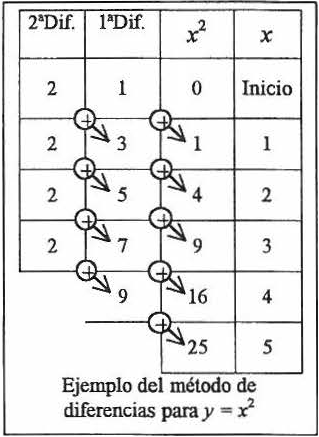
\includegraphics[height=6.2cm]{imgs/MDTable}
	\caption{La máquina de diferencias (1822) desempeñaba la función de tabular polinomios con la última 
	diferencia constante, suscitó un gran interés público, y Babbage se vio envuelto en un ambicioso 
	proyecto en colaboración con el gobierno.}
	\label{fig:mdif}
\end{figure}

El objetivo de la máquina de diferencias era producir tablas numéricas libres de error, una de las 
principales necesidades estratégicas del mayor imperio marítimo de la época, debido a que las tablas 
logarítmicas contenían errores. La máquina analítica se benefició de la experiencia de Babbage con este 
proyecto, principalmente del instrumento teórico que había desarrollado para representar todas las 
interacciones entre las piezas móviles de una máquina en cada ciclo de operación: la notación mecánica, 
esta permitía inventar nuevas máquinas y simplificarlas o comprobar el correcto funcionamiento de la misma.

Empleando ideas usadas en la máquina de diferencias Babbage se planteó llegar a una máquina más general, 
debido a la existencia de números tabulares útiles como los trigonométricos o los logarítmicos, primeramente 
se intentó hacer modificaciones al eje que representaba la diferencia constante en la máquina, pero esto 
no era suficiente, Babbage llegó a la conclusión que eran necesario mecanismos multiplicadores y divisores 
y por tanto era imprescindible extender el modelo actual que se tenía para la totalidad del análisis 
matemático. 

\subsection*{Almacenamiento y Operaciones Aritméticas}

El diseño general de la máquina analítica sigue principios muy distintos, los elementos principales de 
almacenamiento y transmisión numérica están basados en ejes de ruedas numeradas y dentadas comunicados 
por engranajes de forma similar a máquina de diferencias, existen algunas características agregadas 
además de modificaciones para mejorar el cálculo.

Para definir la máquina analítica Babbage seleccionó el sistema decimal debido a que facilitaba la 
multiplicación y división. Además se definió por primera vez el término de almacenar un valor, esto 
se hacia mediante un engranaje, donde su posición representaba el número almacenado, en la 
Fig.~\ref{fig:SaA} a la izquierda se muestra como se almacenaban los valores, en la parte derecha el 
mecanismo base de la suma, este fue modificado para mejorarlo, entre las mejoras se encontraba la 
\emph{llevada anticipada (Anticipating Carry)} $^{\cite{bromley}}$ la cual mejoraba considerablemente la velocidad
de operaciones.

\begin{figure}
	\centering
	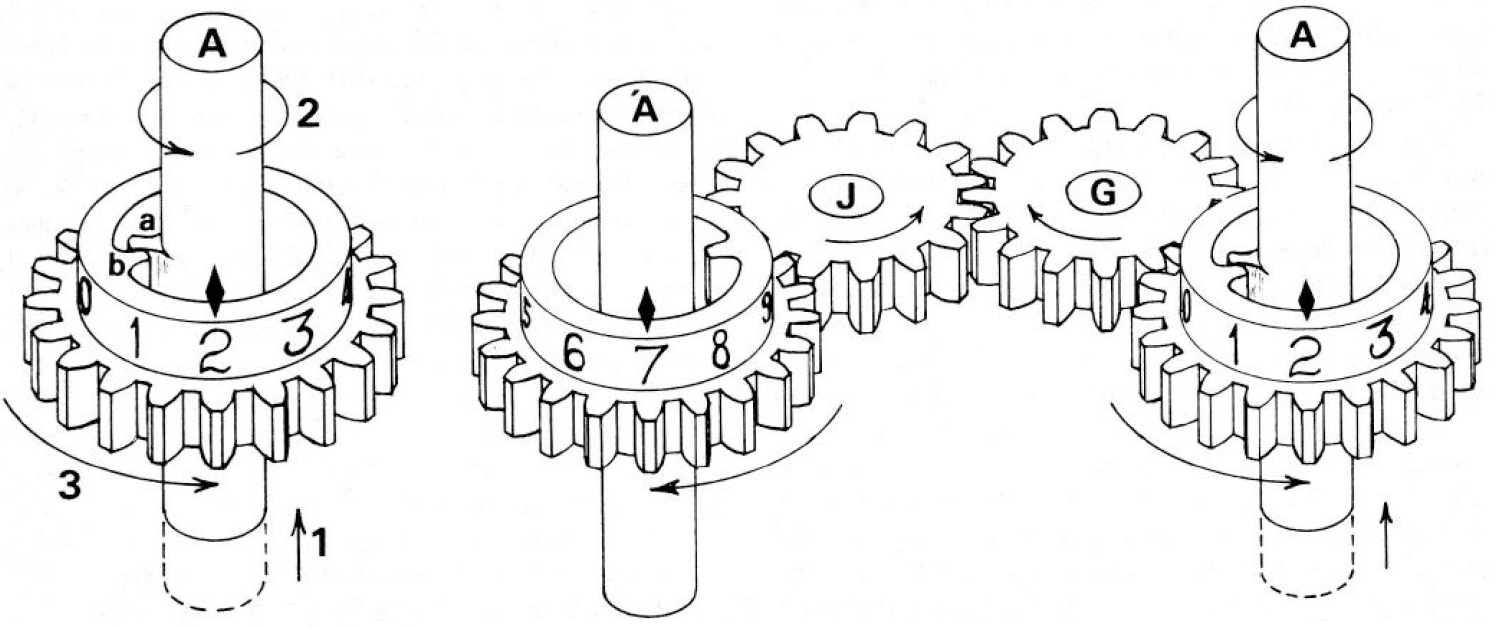
\includegraphics[height=5.1cm]{imgs/SaA}
	\caption{A la izquierda un eje para almacenar un dígito decimal, el proceso de lectura consumía 
	la información en el eje. A la derecha el modelo de suma básico sin llevada}
	\label{fig:SaA}
\end{figure}

Para leer un número era necesario realizar el movimiento del engranaje tantas veces como el número 
almacenado, por tanto el proceso de lectura era destructivo, ya que implica la reducción a cero del eje 
leído, algunos ejes tendrán un doble juego de ruedas numeradas acompañado por un sistema de transmisión 
circular, que permite volcar el número en el segundo juego de ruedas numeradas al mismo tiempo que se lee 
el número del primero, esto se aprecia en los ejemplo de suma avanzada $^{\cite{giudice}}$ y multiplicación.

Para sumar podemos observar la parte derecha de la Fig.~\ref{fig:SaA}, donde se ve como los engranajes 
\verb*|J| y \verb*|G| realizan el proceso de suma, moviendo el eje $'\verb*|A|$ en sentido aditivo y \verb*|A| 
en el sentido substractivo. Es fácil observar como si en $'\verb*|A|$ esta representado un número distinto de 
cero entonces en \verb*|A| se almacena la suma de los números de ambos ejes debido al sentido de los 
engranajes. Evidentemente en este modelo no se toma el cuenta la llevada en caso de los dígitos del número, 
esta será comentada más adelante.

Una de las nuevas características agregadas para la máquina analítica fue la multiplicación y división, 
La transmisión entre ejes puede engranarse o desengranarse automáticamente según las necesidades del 
cálculo. Algunos de estos engranajes pueden alterar la transmisión cambiando la posición decimal del 
número transmitido, de esta forma se dividía y multiplicaba por 10 de forma sencilla.

\begin{figure}
	\centering
	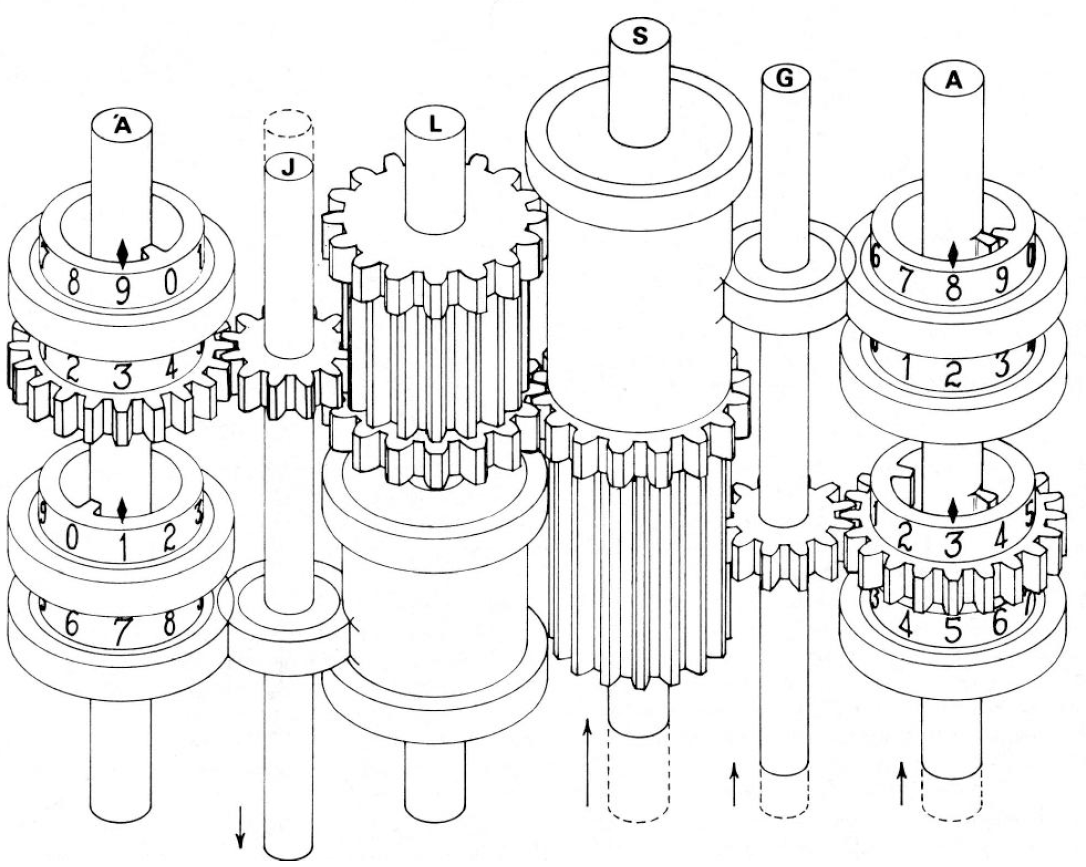
\includegraphics[height=6.1cm]{imgs/Mult}
	\caption{El mecanismo de multiplicación se sustentaba en los engranajes L y S los que al moverse permitían de forma 
	fácil multiplicar o dividir por 10}
	\label{fig:Mult}
\end{figure}

Los movimientos realizados sobre los pistones largos \verb*|S| y \verb*|L| permitían multiplicar y 
dividir por 10 de forma rápida. Como se vio en la suma era necesario una forma de llevar el valor extra 
cuando se esta operando, esta llevada fue representada de forma simple mediante una advertencia de 
llevada la cual se activaba cuando se alcanzaba el dígito 9 en el eje, de esta forma se sabía que 
era necesaria una rotación más en el próximo eje, en la Fig.~\ref{fig:Carry} en la parte de la izquierda 
se puede apreciar este mecanismo.

\begin{figure}
	\centering
	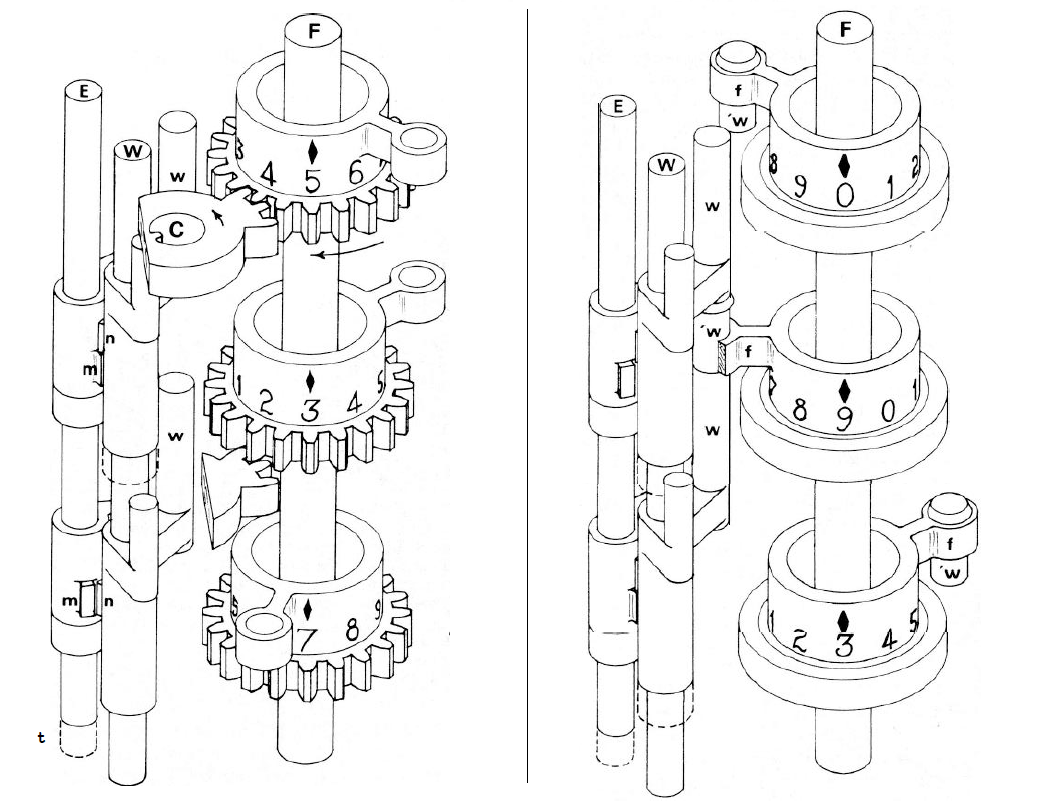
\includegraphics[height=6.1cm]{imgs/Carry}
	\caption{A la izquierda se tiene el mecanismo de llevadas sin anticipación, el mecanismo de la derecha es el resultado de modificar \textbf{w} para poder determinar todas las llevadas antes de iniciar la operación}
	\label{fig:Carry}
\end{figure}

Podemos notar como, cada vez que hay una llevada secuencial , es necesario volver a activar la
alerta, esto resta en velocidad, Babbage pronto sustituyó este sistema de llevadas secuenciales el cual 
se había hecho en la máquina de diferencia, por un mecanismo capaz de registrar en un solo paso las
llevadas necesarias tras una suma en cada nivel decimal, propagando todas las llevadas en el paso siguiente. 
Este se llamó \emph{llevada anticipada}. En números de 40 cifras, este sistema puede acelerar hasta un 
400 \% las operaciones aritméticas. En la Fig.~\ref{fig:Carry} en su parte derecha se puede apreciar como 
el vértice \verb*|w| que antes se encontraba en porciones ahora es completo, de esta forma y con la conexión 
con la pieza \verb*|f| se podía anticipar las llevadas a partir de las unidades que serían realizadas en 
la operación.

\subsection*{Estructura y Funcionamiento de la Máquina Analítica}

La máquina analítica realiza una separación en su estructura que es paralela a la separación moderna entre 
la unidad de procesamiento CPU y una unidad de almacenamiento en este caso la RAM, obviamente en la 
actualidad estos modelos son más avanzados Babbage definió ya desde el siglo XIX el modelo base que se 
emplea en contemporaneidad.

Babbage dividió su máquina en dos unidades el \emph{almacén} y \emph{molino}. El almacen se componía de un
número indefinido de ejes simples de ruedas numeradas todo ellos conectados a una cadena de transmisión de 
la que pueden desengranarse cuando sea necesario. En el molino los números son operados aritméticamente 
según un patrón preestablecido por el sistema de control, este se disponía en torno a unos grandes engranajes 
o ruedas centrales que comunican todo el conjunto, y se componía básicamente de dos ejes numéricos, el eje
de cabeza y eje de cola, donde se operan las cantidades $^{\cite{giudice}}$. Además, sobre las ruedas centrales hay 9 ejes tabulares, donde alojar los 9 múltiplos de una cantidad al dividir o multiplicar, estos ejes disponen de 
transmisión circular para no perder la información al ser leídos y para mover sus posiciones decimales 
cuando convenga. También tiene dos ejes numerados para comunicarlo con el almacén, un eje es para la salida
y el otro para la entrada de valores al almacén.

La máquina cuenta con un sistema de control de doble nivel, ya que un nivel implementaba los algoritmos necesarios
para las cuatro operaciones y otro controlaba la sucesión de operaciones a realizar además de determinar cuales 
ejes del almacén había que leer o escribir en cada momento, estos controles eran el aritmético y algebraico 
respectivamente. El mecanismo para ambos sistemas de control era del mismo tipo, el tambor y el aparato reductor.
Análogo al mecanismo de las cajas de música, se distingue de este en que los tacos pueden atornillarse a mano para ser modificados y que ejercen su acción por el desplazamiento horizontal del tambor sobre una columna de palancas sensoras,
la acción de cada palanca revertía en la disposición de diversas partes de la máquina analítica, entre estas se incluye el movimiento tanto circular como rectilíneo de los tambores. Del mismo modo, el propio tambor, gracias al aparato reductor que lo desplaza y las palancas lectoras, puede cambiar su acción en virtud de ciertos eventos predeterminados en el funcionamiento de cualquier parte de la máquina, esto proporciona una libertad algorítmica total, con recursividad y condicionalidad completas. Pero en 1836 Babbage, limitó los tambores solamente a la ejecución de las operaciones aritméticas e introdujo las tarjetas perforadas para el control algebraico y la entrada, salida y almacenamiento de números. Las tarjetas tenían la ventaja de albergar una cantidad ilimitada de órdenes
y eran mucho más fáciles de manejar que los pesados tambores, en la próxima sección veremos como se empleaban las
tarjetas perforadas para programar la máquina analítica.

\begin{figure}
	\centering
	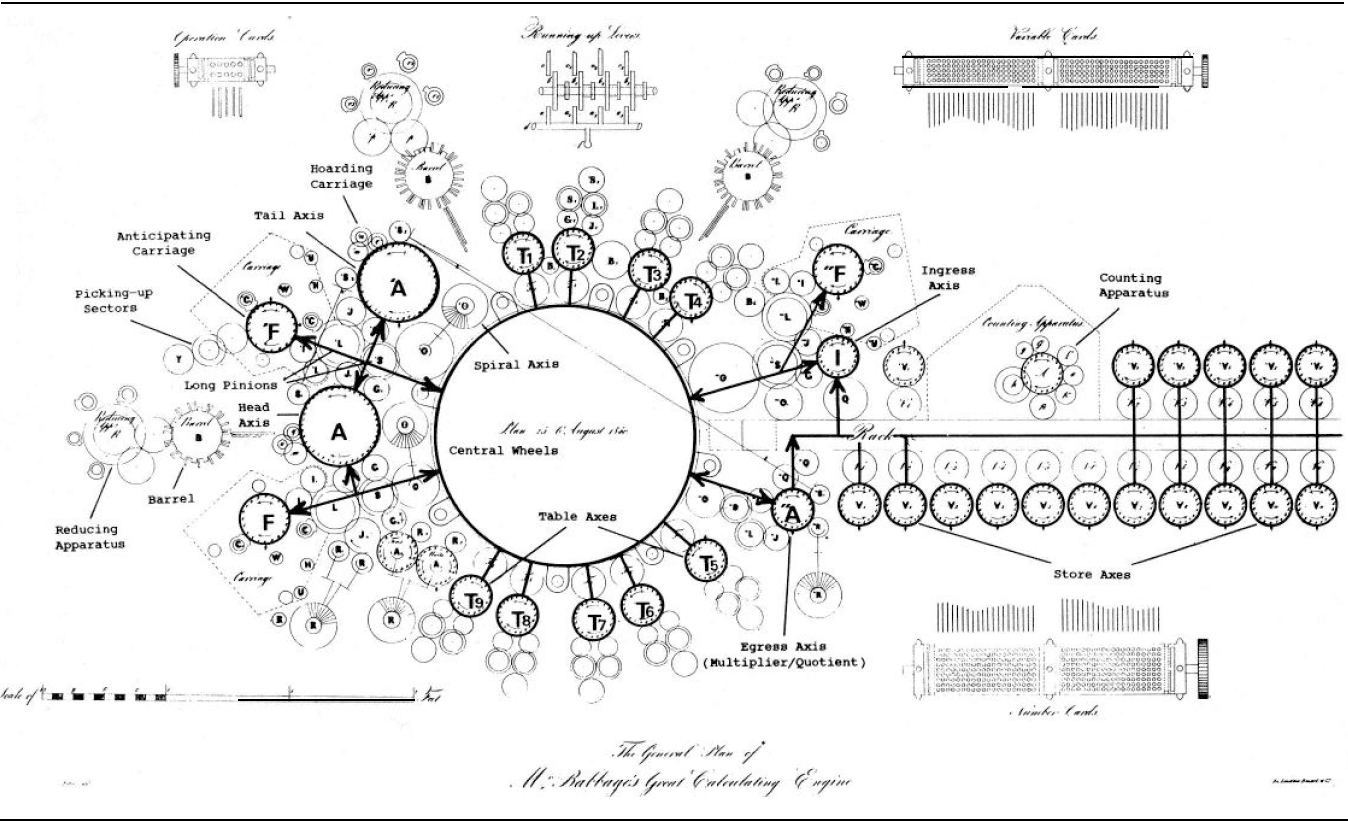
\includegraphics[height=7.4cm]{imgs/AMachine}
	\caption{Muestra los planos realizados por Babbage, las componentes Vn representan los ejes que componen el almacén, la unidad de control se encuentra en el centro, mientras alrededor se hallan los mecanismos para la operaciones aritméticas y los tambores usados para la multiplicación T1-T9, junto a los cabezales y los mecanismos de llevada}
	\label{fig:AM}
\end{figure}

La Fig.~\ref{fig:AM} muestra el plano de la máquina analítica de Babbage, las zonas resaltadas constituyen las principales componentes que intervenían en la ejecución y serán explicadas en esta sección, además se aprecian otras componentes secundarias. A la derecha se encuentran los ejes $\verb*|V|_{\verb*|n|}$ estos forman el almacen, estos pueden ser referenciados en las tarjetas perforadas para ser empleados en las operaciones, asi una vez que se desea usar el valor almacenado en el eje se realiza un volcado $\verb*|V|_{\verb*|n|} \rightarrow  \verb*|I|$, donde \verb*|I| es el eje de ingreso, desde aquí el valor es enviado mediante las ruedas centrales al eje de cabeza \verb*|A|, donde es sumado o restado al número que allí hubiera almacenado. Un problema fundamental en este proceso es la imposibilidad de emplear el dispositivo de llevadas indistintamente para la suma y la resta, esto es solucionado conectando el eje \verb*|A| con los dos aparatos de llevadas \verb*|F| y $'\verb*|F|$ de manera que $'\verb*|F|$ efectúa las llevadas de las sumas en \verb*|A|, mientras que \verb*|F| hace las llevadas de las restas. Si el resultado parcial debe ser almacenado, es enviado desde el eje de cabeza \verb*|A| hasta el eje de salida $''\verb*|A|$, desde donde se envía a su eje de almacén en el cual debe ser almacenado. 

Este proceso de suma y resta resulta lento Babbage propuso que la máquina hiciera simultáneamente los cuatro pasos sucesivos para las operaciones mediante un método bastante parecido a lo que hoy conocemos como \emph{pipeline}. Mientras el primer valor sumado se devuelve al almacén, el siguiente resultado se introduce en el eje de salida $''\verb*|A|$, al mismo tiempo los ejes de cabeza y cola se encuentran sumando el próximo resultado mientras el eje de ingreso \verb*|I| esta recibiendo el próximo operando.

El proceso de obtención de datos ocurría de forma similar a la suma y resta para la multiplicación esta vez se leían dos
valores y eran almacenados en los ejes \verb*|A| y $'\verb*|A|$ donde son comparados, el menor se almacena en el eje de 
salida $''\verb*|A|$, desde donde será usado como multiplicador, con el multiplicando se genera una tabla de múltiplos 
en los ejes tabulares $\verb*|T|_{\verb*|1|}$-$\verb*|T|_{\verb*|9|}$ mediante sumas sucesivas realizadas de forma directa con el eje de ingreso 
\verb*|I|. La multiplicación se inicia por las unidades del multiplicador acorde a ese número se selecciona el múltiplo $\verb*|T|_{\verb*|n|}$ correspondiente al multiplicando, este múltiplo es sumado en los ejes \verb*|A| y $'\verb*|A|$, realizando las llevadas empleando a $''\verb*|F|$. luego se mueven las posiciones decimales de los ejes de tabla $\verb*|T|_{\verb*|n|}$ y se reinicia el proceso con las decenas del multiplicador, así continúan los ciclos hasta que el resultado esta listo y es enviado al 
almacén.
\newpage

\subsection*{Programando la Máquina Analítica}

El funcionamiento de la máquina analítica requería realizar una programación para definir que ejes del almacen, que operaciones y en que orden serían realizados con estos y finalmente reportar o almacenar los resultados. Para esto se
emplearon las tarjetas perforadas, estas eran el recurso con el que se contaba para realizar la programación y fue descrito por Ada Lovelace en \cite{lovelace}

Las tarjetas tenían varios fines, las encargadas del control algebraico tenían tres tipos: las tarjetas de variable, las tarjetas de operación y las tarjetas de combinatorias y de índice. Por otro lado existían tarjetas numéricas con las que se podía introducir cantidades en el almacén de modo automático, estas contaban con 9 filas y 41 columnas, cada columna representa un dígito del número, excepto la última, que es el signo algebraico $^{\cite{bromley}}$, las perforaciones por columna indicaban el dígito, de esta forma se desaprovechaba espacio de almacenamiento pero al emplear el sistema decimal se ganaba eficiencia a la hora de leer los números, la máquina también podría perforar tarjetas numéricas como medio de almacenamiento externo.

Las tarjetas se disponían unidas entre si por hilos, el control algebraico de la máquina necesitaba dos cadenas de
tarjetas relacionadas, primeramente una cadena se conformaba por tarjetas de operación, donde cada una simbolizaba una
operación algebraica en esta cadena se intercalaban en caso que sea necesario tarjetas combinatorias y de indice para 
la ejecución de bucles previstos en el algoritmo a seguir. La segunda cadena representa las tarjetas variables que hacen referencia a las columnas del almacén implicadas en cada operación sucesiva ordenada por la primera cadena. Una
limitación importante era que en este punto Babbage no tenia el concepto de dirección de memoria que tenemos hoy en día
además de que era muy complicado en ese momento calcular de forma automática que ejes del almacén debían ser usados 
para la operación. El empleo de este juego de tarjetas era difícil de construir para cálculos complejos pero aun así
con este enfoque se poseía una gran generalidad matemática a la hora de los cálculos.

Para comprender como funcionaba la máquina analítica usaremos el ejemplo empleado por Ada Lovelace en \cite{lovelace}, en el cual representa los estados de los distintos ejes del almacén, el estado de la máquina en cada operación además de las diferentes variables que intervienen.

Debemos resolver el sistema de ecuaciones de dos variables con dos incógnitas siguiente:

\begin{equation}
	\left\{
		mx + ny = d \atop
		m'x + n'y = d'
	\right.
\end{equation} 

Resolviendo este sistema obtenemos:

\begin{equation}
	x = \frac{dn' - d'n}{n'm - nm'}
\end{equation}

De forma análoga puede obtenerse $y$, ahora representemos los valores de los coeficientes en los distintos ejes $\verb*|V|_{\verb*|n|}$ de la siguiente forma: $\verb*|V|_{\verb*|0|} = m$, $\verb*|V|_{\verb*|1|} = n$, $\verb*|V|_{\verb*|2|} = d$, $\verb*|V|_{\verb*|3|} = m'$, $\verb*|V|_{\verb*|4|} = n'$, $\verb*|V|_{\verb*|5|} = d'$, $\verb*|V|_{\verb*|6|} = n$ y $\verb*|V|_{\verb*|7|} = n'$.\footnote{Los valores de $n$ y $n'$ se almacenan repetidos debido a que son necesarios para más de una operación, de esta forma no es necesario leer nuevamente a mitad de la ejecución} Las operaciones a realizar y el orden se establece mediante las
tarjetas de operaciones y ordenamiento, la tabla de la Fig.~\ref{fig:stable} muestra como sería el proceso de cálculo
además podemos ver en que ejes quedarán almacenados los resultados en cada parte del proceso.

\begin{figure}
	\centering
	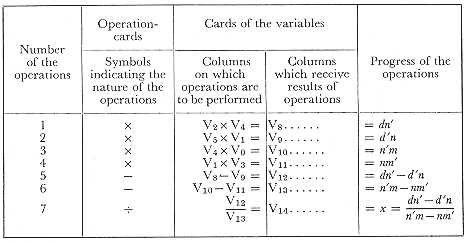
\includegraphics[height=6.4cm]{imgs/stable}
	\caption{Tabla simplificada empleada para la creación de las tarjetas perforadas empleadas en la programación de la máquina analítica. Tomada de \cite{lovelace} como explicación de la solución de un sistema de ecuaciones lineales}
	\label{fig:stable}
\end{figure}

Empleando las tarjetas de variable podemos decir para cada operación que ejes serán usados y en cual será almacenado el resultado final, esto iría en el segundo hilo de tarjetas que procesa la unidad de control. En el primer hilo colocamos 
las operaciones que se realizarán para los valores que vamos sacando del almacén, en este caso no solo es necesario colocar tarjetas de operaciones, sino es necesario poner tarjetas de ordenamiento debido a que tenemos que hacer dos restas antes de la división. La Fig.~\ref{fig:ltable} muestra de forma detallada el estado de los ejes, la cantidad 
de dígitos y todas las operaciones que se realizan para llegar a los valores de $x$ y $y$.

\begin{figure}
	\centering
	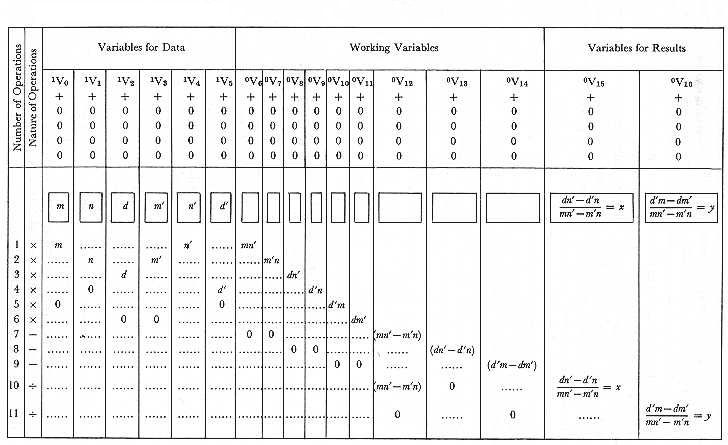
\includegraphics[height=7.4cm]{imgs/ltable}
	\caption{Muestra los dígitos y signo por defecto para cada eje, además cada fila representa los valores que se encuentran en los ejes una vez que completa una operación. Se clasifica los ejes del almacén en variables de entrada, temporales y de salida}
	\label{fig:ltable}
\end{figure}

En la Fig.~\ref{fig:ltable} se puede apreciar como con la máquina analítica se introdujo el concepto de variable temporal ya que era necesario almacenar determinados cálculos con el fin de reutilizarlos, podemos entonces distinguir entre las tarjetas variables varios tipos, aquellas que representaban la entrada o sea los datos del problema, las temporales las cuales se empleaban para resultados intermedios y las de salida, estas podían referirse al almacén o a una tarjeta perforada resultante de la impresión de la máquina. 

\newpage

En \cite{lovelace} Ada Lovelace explica como es posible el empleo de la máquina analítica para resolver sistemas de ecuaciones como el que vimos, polinomios, funciones trigonométricas e incluso integrales, también define conceptos como ciclo los cuales aparecian constantemente en determinados cálculos. Además muestra como calcular los números de Bernoulli, introduciendo la noción de condicional a la hora de definir como debían crearse las tarjetas perforadas.
De esta forma Ada Lovelace ya desde 1843 introduciría conceptos tan comunes hoy en día en la programación como son las variables, ciclos entre otros.

\begin{thebibliography}{4}

\bibitem{giudice} Giudice, J.P.: \textit{Complejidad y Dimensiones en los
Estudios sobre Babbage: La Máquina Analítica}, Universidad del País Vasco.

\bibitem{bromley} Bromley, A.G.:\textit{ Charles Babbage’s
Analytical Engine}. 

\bibitem{francis} Francis, J., Fuegi, J.: \textit{Lovelace and Babbage and the Creation
of the 1843 "Notes"}

\bibitem{lovelace} Lovelace, A.A., Menabrea, L.: \textit{Sketch of the Analytical Engine invented
by Charles Babbage} (1843) By L.F. Memabrea, of Turin, officer of the Military
Engineers, with notes upon the memoir by the translator. Usamos la versión
editada en: Campbell-Kelly, M. (ed.) (1989) The Works of Charles
Bahhage. Vol. 3, cap. VII. Nueva York, New York University Press.

\bibitem{nytimes} Miller, C.C., \textit{Ada Lovelace, la matemática que allano el camino a la programación}, The New York Times, \url{https://www.nytimes.com/es/2018/03/10/espanol/cultura/ada-lovelace-obituario-overlooked.html}

\bibitem{url} Computer History Museum: Charles Babbage, \url{https://www.computerhistory.org/babbage/charlesbabbage/}

\bibitem{wiki} Wikipedia: Charles Babbage, \url{https://es.wikipedia.org/wiki/Charles_Babbage}

\end{thebibliography}

\end{document}
